\chapter{Mobile Networks}
The mobile telephones were at first introduced in the 60s, but were not so popular and required an
operator to connect the calls. Ever since, the technology has swiftly evolved, and now we have
smartphones, which are able to do many other things outside voice calls, and today there are even
more mobile phones than people in the world.\\ 
All those device are connected trough Mobile Networks, which allow radio user terminals , named User
Equipment(UE) or Mobile Stations(MS), to connect to global networks infrastructure, like the
Internet. A mobile network is divided into two parts: the \textbf{Radio Access Network}(RAN), which
is The part of the network that connects the UE to the core network, and the \textbf{Core
Network}(CN) itself, which is the part of the network that connects the RAN to the global network
infrastructure.\\
\begin{figure}[h]
  \centering
  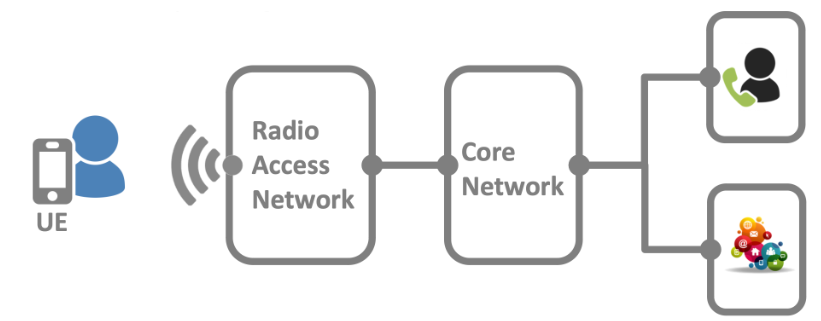
\includegraphics[width=0.5\textwidth]{img/wireless/mobile network overview.png}
  \caption{The overview of a mobile network}
  \label{fig:mobile-network}
\end{figure}
In the 2G and 3G technologies, the CN that provided access to the telephone service is based on
circuit-switched technology, which means that the connection between the two users is established
before the communication starts, and a separate core network is based on packet-switched technology,
to provide internet access. This was reverted after the 4G technology, in which the CN is based on
packet-switched technology to provide both telephone and internet services.\\
The main architectural elements of RAN are Base Transceiver Stations (BTS or BS) that
connect to UEs through a radio interface. For the newers technologies, like 4G and 5G, the BTS are
connected directly to the CN, but for the older ones, like 2G and 3G, the BTS are connected to an
additional radio controller placed between the BTS and the CN.\\
\begin{figure}[h]
  \centering
  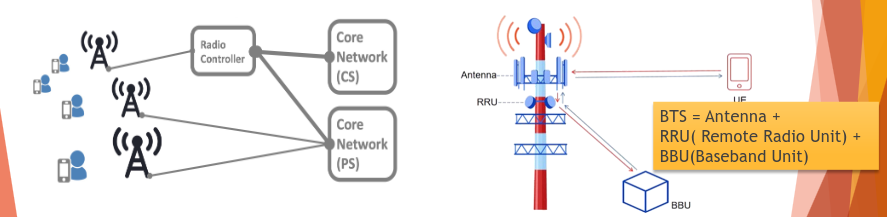
\includegraphics[width=0.7\textwidth]{img/wireless/mobile base stations.png}
  \caption{An overview of the placement of the base stations}
  \label{fig:mobile-architecture}
\end{figure}
\begin{section}{Cellular network Cells}
  Nowadays, the BSs are placed practically everywhere, because the SNR scales quadratically with the
  distance, to provide connectivity at any position, and the UEs can connect to the most convenient
  BS, which is usually the closest one. The area covered by a BS is called a \textbf{cell}.\\
  Historically, the cells share is considered \textit{hexagonal}, but in reality they are not, because
  signals do not propagate in a straight line, and the cells are usually irregularly shaped. The
  hexagonal approximation is used to simplify the calculations.
  \begin{subsection}{Frequency reuse}
    Radio waves are a limited resource, and the same frequency cannot be exclusively dedicated to a
    channel in a cell. But if the same frequency is reused, which is the basic idea, it generate
    interference, which is not ideal, so the cells are divided into \textbf{clusters}, which allows
    to reuse frequencies provided that the interference is limited and constrained. Each cluster
    have a pattern, that can be repeated for each cluster without generating too much interference.
    After all, if we consider a individual cell to have homogeneous traffic, and $k$ frequencies
    have to be assigned between a group of cells, you can notice that this problem is reducible to a
    \textbf{graph coloring problem}, which is NP-hard.
  \end{subsection}

  \begin{subsubsection}{Cell sizes}
    There are actually different sized of cells, which are used to provide different coverage and
    capacity. 
    \begin{itemize}
      \item \textbf{Macrocells} are the largest cells, and are used to provide coverage in rural
        areas, where the density of users is low.
      \item \textbf{Microcells} are used to provide coverage in urban areas, where the density of
        users is high, and the cells are smaller to provide more capacity.
      \item \textbf{Picocells} are used to provide coverage in buildings, like offices or shopping
        malls, where the density of users is very high.
      \item \textbf{Femtocells} are used to provide coverage in homes, where the density of users
        issues very high.
    \end{itemize}
    \begin{figure}[h]
      \centering
      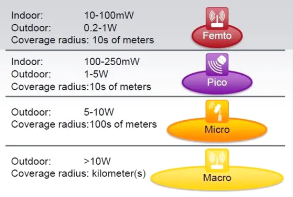
\includegraphics[width=0.4\textwidth]{img/wireless/cell sizes.png}
      \caption{The different sizes of cells}
      \label{fig:cell-sizes}
    \end{figure}
  \end{subsubsection}

  \begin{subsection}{Mobility Management}
    Users are not static in space, but they are able to move freely in the cell, and between cells.
    The network must thus be able to manage the mobility of the users, and to do so it uses a
    mechanism called \textbf{Handover}, tracking the user's position(in term of cell) and changing
    the network to adapt routing and commands to with the connection to the new cell.\\
    \begin{figure}[h]
      \centering
      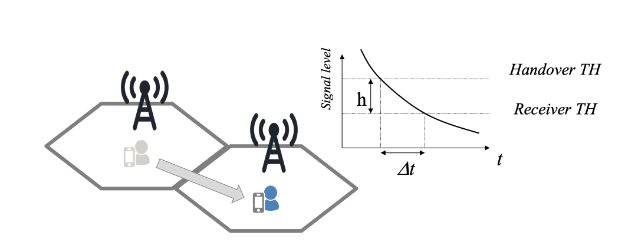
\includegraphics[width=0.5\textwidth]{img/wireless/mobile handover.png}
      \caption{An overview of the handover process}
      \label{fig:handover}
    \end{figure}
    The network is constantly monitored to check the signal strength and the quality of each
    neighboring cell, in respect to the MS, which measurements are sent to the BS every 480ms(at
    least for GMS). When the signal strength of the current cell is drops below a certain
    \textbf{threshold}, or becomes lower than the signal strength of a neighboring cell, the
    handover process is started by sending an \textbf{handover request} to the MS via the BTS which
    is serving the MS. While the MS is preparing, the network sends an \textit{Immediate Assignment}
    message to the MS, which contains the frequency and the time slot to use to connect to the new
    cell, and will be followed by the MS. Once the MS is successfully handed over to the new cell,
    data and voice traffic are transferred to the new cell, and after it is completed by a
    \textit{Handover confirmation} message, the old connection is released.\\
    If the handover process results in a change in the Base Station Controller (BSC) or Mobile
    Switching Center (MSC), new connections are established with the new controllers.The old BSC and
    MSC release resources associated with the call and update their databases with the MS’s new
    location information.
  \end{subsection}

  \begin{subsection}{Mobile Updates}
    The users can still move but not want an handover to be performed, for example when the user is
    moving very fast. In this case, the network is then divided in Location Areas(LAs), which are
    a set of cells. The MS sends a \textit{Location Update Request} to the network, and if the MS 
    change the LA, the position database is updated.\\ 
    This procedure is also very useful to know where the device is, and the process to find out
    exactly where the device is called \textbf{paging}. All base stations in LA broadcast a paging 
    message with the ID of the called user. When the mobile terminal replies, the network knows
    where the device is, and can establish a connection.
    \begin{figure}[h]
      \centering
      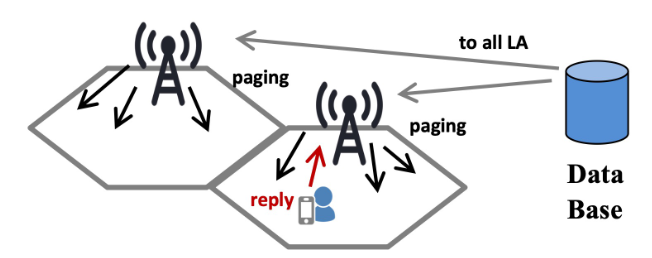
\includegraphics[width=0.5\textwidth]{img/wireless/mobile paging.png}
      \caption{An overview of the paging process}
      \label{fig:paging}
    \end{figure}
    \begin{subsubsection}{Paging vs Location update}
      The larger are the LA, the less frequent are the location updates, but the more frequent are 
      the paging messages. The smaller are the LA, the more frequent are the location updates, but
      the less frequent are the paging messages. The size of the LA is a trade-off between the
      frequency of the location updates and the frequency of the paging messages.
      This also depends on the mobility of the users, and the arrival frequency of the calls.
    \end{subsubsection}
  \end{subsection}
\end{section}

\begin{section}{Signalling}
  Signalling, in mobile networks, is in charge of establishing, maintaining, and terminating a
  service, assigning resources or modify them.
  In a classic telephone service, the signalling is in charge of routing and setting up circuits for
  phones, while in a mobile(IP) network, the signalling is used to set up media sessions.\\
  The basic service provided by signalling is the Basic Call that is used to set up a telephone
  call. Signalling hash two main components: the user signalling and the network signalling.
  \begin{paragraph}{User signalling}
    The user signalling is used to allow communication between user terminals and the network, and
    in particular to:
    \begin{itemize}
      \item ask for a service
      \item indicate the called party
    \end{itemize}
    The required information about the call status are provided by the network.
  \end{paragraph}
  \begin{paragraph}{Network signalling}
    The network signalling is used to allow communication between switching stations, and in
    particular to:
    \begin{itemize}
      \item route calls among the available paths
      \item allocate resources
      \item management operations
    \end{itemize}
    It is also used for providing supplementary services like special numbers(like 911), calling
    party notifications, mobility management, and so on.
  \end{paragraph}
  \begin{figure}[h]
    \centering
    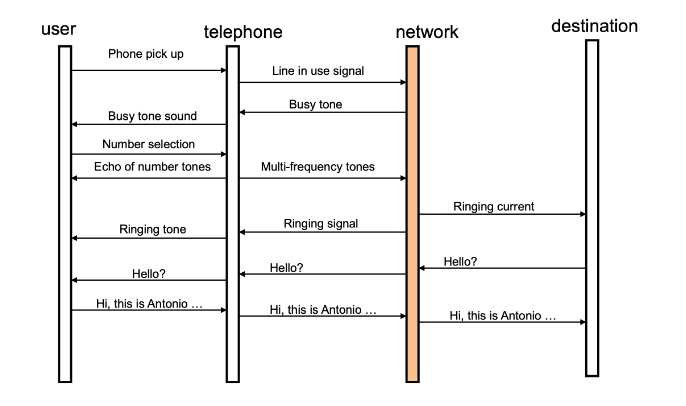
\includegraphics[width=0.6\textwidth]{img/wireless/signalling.png}
    \caption{An overview of the signalling process for a simple call}
    \label{fig:signalling}
  \end{figure}
  \begin{subsection}{Digital user signalling}
    We are now in a digital era, and the user signalling is now digital. ISDN, which stands for
    Integrated Services Digital Network, is a set of communication standards for simultaneous
    digital transmission of voice, video, data, and other network services over the traditional
    circuits of the public switched telephone network. Digital interfaces works in
    a rather different fashion, because the information is sent in digital messages transmitted over
    L2 frames in the D channel of the ISDN interface. The set of protocols for user signalling
    defines the DSS1 signalling system, which are transported directly into LDAP frames.

    \begin{figure}[h]
      \centering
      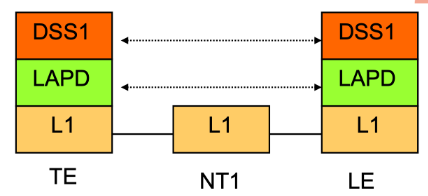
\includegraphics[width=0.4\textwidth]{img/wireless/digital user signalling.png}
      \caption{An overview of the digital signalling process}
      \label{fig:digital-signalling}
    \end{figure}

    \begin{figure}[h]
      \centering
      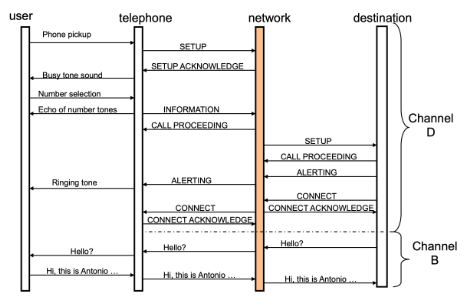
\includegraphics[width=0.5\textwidth]{img/wireless/digital user signalling exhange.png}
      \caption{The exchange of figure \ref{fig:signalling} in digital signalling}
      \label{fig:digital-signalling-2}
    \end{figure}
  \end{subsection}
  
  \begin{subsection}{Network signalling}
    Network signalling is a old standard, but still used today. The,kind of, modern signalling stack
    is called \textbf{SS7}, which stands for Signalling System 7, and is a set of telephony
    signalling protocols used for telephony, and which evolved to support all the services of modern
    fixed and mobile networks.\\
    The signalling is performed out-of-band, meaning that the signalling messages are transmitted
    over a separate network, and not over the same network used for the voice calls, and performed
    via packet switching.\\
    SS7 defines different kind of nodes:
    \begin{itemize}
      \item \textbf{Service Switching Points(SSP)} are the nodes that switch the calls and are
        responsible for the call control. They convert global titles digits(ie. phone numbers) into
        ss7 signalling messages.
      \item \textbf{Service Control Points(SCP)} are the nodes that provide application access to
        the network, and are responsible for the service logic.
      \item \textbf{Signal Transfer Points(STP)} are the nodes that route the messages between the
        SSPs and SCPs, and are responsible for the routing of the messages.
    \end{itemize}

    \begin{figure}[h]
      \centering
      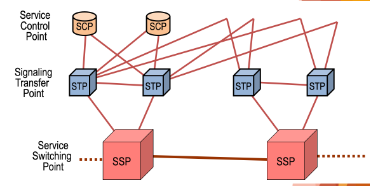
\includegraphics[width=0.5\textwidth]{img/wireless/ss7 architecture.png}
      \caption{An overview of the SS7 architecture}
      \label{fig:ss7}
    \end{figure}

    For the datagram packet switched network, The lower part of the SS7 protocol stack includes:
    \begin{itemize}
      \item Physical layer(MTP-1) defines the physical and electrical characteristics of the
        signalling links of the SS7 network, Signalling links utilise DS–0 channels and carry raw
        signalling data at a rate of 56 kbps or 64 kbps.
      \item Data link layer(MTP-2) provides link-layer functionality, in particular reliability
        and error detection.
      \item Network layer(MTP-3) provides routing functionality, and ensures that messages can be
        delivered between signalling points across the SS7 network regardless of whether they are
        directly connected. It also provides capabilities like node addressing, routing, alternate
        routing, and congestion control.
    \end{itemize}

    \begin{figure}[h]
      \centering
      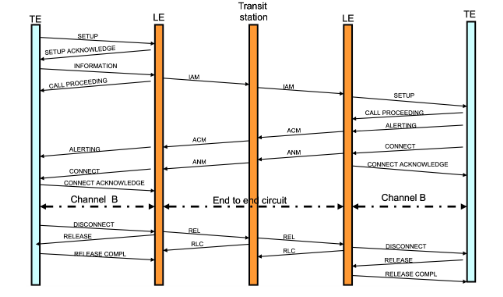
\includegraphics[width=0.5\textwidth]{img/wireless/ss7 digital call.png}
      \caption{The same call of figure \ref{fig:signalling} by the ss7 point of view}
      \label{fig:ss7-call}
    \end{figure}
    \begin{subsubsection}{Security in ss7}
      SS7 was designed in an era when security concerns were not considered. Every node in the SS7
      is trusted, because no authentication is performed, and the messages are not encrypted. 
      A lot of nasty attack can be performed, like:
      \begin{itemize}
        \item \textbf{Location tracking} by sending a location request to the network, and the
          network will reply with the location of the user.
        \item \textbf{SMS interception} by sending a SMS request to the network, and the network will
          reply with the SMS.
        \item \textbf{Call interception} by sending a call request to the network, and the network
          will reply with the call.
        \item \textbf{Denial of service} by sending a lot of messages to the network, and the network
          will be overloaded.
        \item \textbf{Fraud} by sending a call request to the network, and the network will reply
          with the call, but the call will be charged to the victim.
      \end{itemize}
      All those attacks are still possible today.
      \begin{figure}[h]
        \centering
        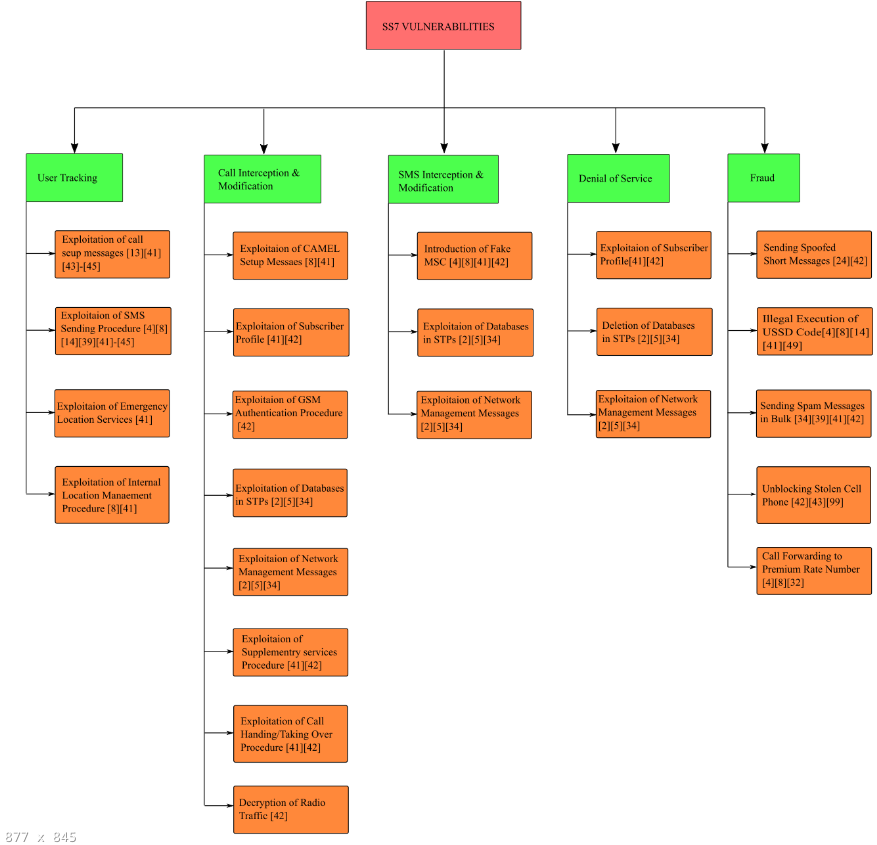
\includegraphics[width=0.5\textwidth]{img/wireless/ss7 attacks.png}
        \caption{An overview of the SS7 attack}
        \label{fig:ss7-attack}
      \end{figure}
    \end{subsubsection}
  \end{subsection}
\end{section}

\begin{section}{GSM network}
  The first network architecture of GSM was for circuit switched (CS) services only, and telephone
  service in particular. It was mainly divided into three parts( the UE, the RAN, and the CN), and 
  the CN was divided into three parts: 
  \begin{itemize}
    \item \textbf{Mobile Switching Center(MSC)} is the equivalent of a telephone station for the
      mobile network and includes all control and signalling functions for managing calls and
      mobility
    \item \textbf{Visitor Location Register(VLR)} is a database that contains information about all
      the mobile terminals currently located in the area controlled by the MSC
    \item \textbf{Home Location Register(HLR)} is a database that contains information about all the
      mobile terminals that are registered in the network. It also includes an AuC (Authentication
      Centre) for security procedures
    \item \textbf{Gateway MSC(GMSC)} is the MSC connecting the mobile network to the external
      telephone networks (PSTN) and that implements all signalling interworking functions
  \end{itemize}
  while the RAN was divided into two parts:
  \begin{itemize}
    \item \textbf{Base Transceiver Station(BTS)} is the GSM base station that manages physical layer
      connections with the UEs and the BSC and executes resource allocation commands received by the
      BSC
    \item \textbf{Base Station Controller(BSC)} is the GSM controller that implements higher layer
      protocols and manages all transmission resources of the connected BTSs
  \end{itemize}
  the UM radio intermace of GSM is based on the TDMA technology, but because it still uses the
  classical telephone transport network, the achievable data rate is limited to 65 kbps, and 2048
  Mbps while using E1 links.\\

  \begin{figure}[h]
    \centering
    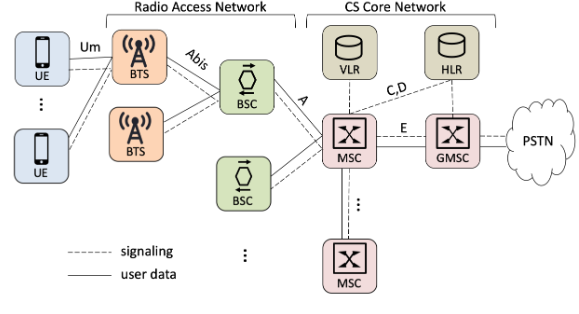
\includegraphics[width=0.5\textwidth]{img/wireless/gsm network.png}
    \caption{An overview of the GSM architecture}
    \label{fig:gsm-architecture}
  \end{figure}
  Of course, signalling is not very efficient, so schanging the infrastructure to a packet-switched
  network is a good idea. The first step was to introduce the GPRS, which stands for General Packet
  Radio Service, which is a packet-switched technology that allows the transmission of data over the
  GSM network. The GPRS network adds some new elements to the GSM network:
  \begin{itemize}
    \item \textbf{Serving GPRS Support Node(SGSN)} is an IP router which plays the same role as the
      MSC in the circuit- switched core, while also having additional functionalities for the
      management of the interfaces and protocols towards the BSS
    \item \textbf{Gateway GPRS Support Node(GGSN)}
  \end{itemize}
\end{section}

\begin{section}{UMTS networks}
  UMTS, or Universal Mobile Telecomunication System, focused on the introduction of better data
  services, by defining a new achitecture, separating the signalling protocols and procedures
  related to the radio access network and those related to the core network to allow future
  evolutions of the core network independent from the access network.\\

  Take a look at the figure \ref{fig:umts-architecture}, you can see that the radio part has been
  modified:
  \begin{itemize}
    \item \textbf{Node B} is the UMTS base station responsible for all functions required for
      sending and receiving data over the air interface( which is based on CDMA). Allocation
      commands received by the RNC. Is also responsible for the power control of all connections
    \item \textbf{Radio Network Controller(RNC)} is the main element of the UTRAN, responsible for
      controlling radio resources of all Node-Bs and mobility. 
  \end{itemize}

  \begin{figure}[h]
    \centering
    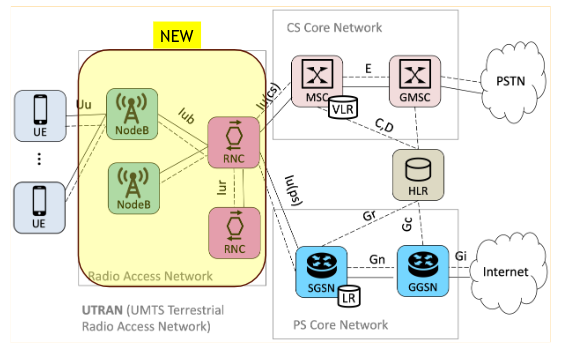
\includegraphics[width=0.5\textwidth]{img/wireless/umts architecture.png}
    \caption{An overview of the UMTS architecture}
    \label{fig:umts-architecture}
  \end{figure}
  The architecture was also modified in the core network, which changed the circuit-switched
  part even for voice calls. The switches became media gateways, which are ip based(VoIP), but
  signalling is still needed.\\
  \begin{figure}[h]
    \centering
    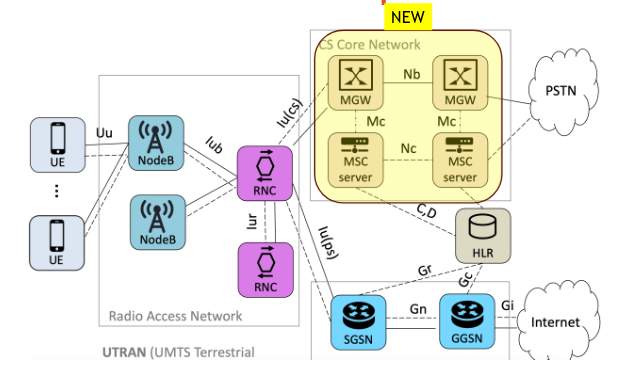
\includegraphics[width=0.5\textwidth]{img/wireless/umts 2.png}
    \caption{The changes in the core network of UMTS}
    \label{fig:umts-core}
  \end{figure}
  The result is that 2G and 3G networks are now fully integrated, and the same network can provide
  both voice and data services.\\

  \begin{subsection}{Implementational Details}
    In GMS, multiple access is based on FDM or TDM, with channels of 200 kHz, while are further 
    split into smaller channels of 45MHz, separating the uplink and downlink. A time slot is 577
    $\mu$s long, and each device can transmit for 8 time slots, or 4.615 ms.\\
    It implements frequency hopping to avoid interference, and power control to be power efficient.
    One of the main issue is synchronization, because of TDMA, because of the delay and the slot
    offsets. Signalling is also a problem, because of the need of a lot of messages to establish a
    call. Its still based on SS7, but because now the network is packet-switched, support for mobile
    signalling is added via a Mobile Application Part(MAP) protocol.\\
    \begin{figure}[h]
      \centering
      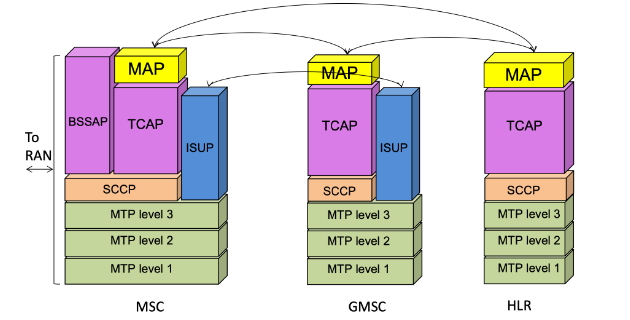
\includegraphics[width=0.5\textwidth]{img/wireless/mobile ss7.png}
      \caption{How MAP was added to the SS7 stack}
      \label{fig:mobile-ss7}
    \end{figure}
  \end{subsection}

\end{section}

\begin{section}{4g}
  In the 4th generation of mobile networks, everything is based on IP, even signalling, meaning that
  signalling is now performed over the same network used for the voice and data traffic. The
  architecture was simplified, being built from scratch, implementing a new "flat" architecture.
  The radio interface was also modified, and the new radio interface supports different bandwidths
  (from 1.25 to 20 MHz) and frequencies.

  \begin{figure}[h]
    \centering
    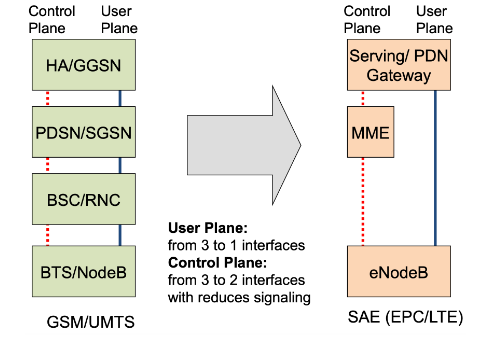
\includegraphics[width=0.5\textwidth]{img/wireless/4g evolution.png}
    \caption{The evolution of the mobile networks}
  \end{figure}
  \begin{subsection}{SAE}
  \end{subsection}

\end{section}
